\documentclass[12pt]{article}

\usepackage{graphicx}
\usepackage{comment}
\usepackage{amsmath}
\usepackage{listings}
\usepackage[labelfont=bf]{caption}
\usepackage[hidelinks]{hyperref}
\usepackage[utf8]{inputenc}
\usepackage[T1]{fontenc}
\usepackage{geometry}
\geometry{a4paper, left=58pt, right=58pt, textwidth=30pt}

\captionsetup{aboveskip=0pt, belowskip=1pt}




\title{%
	{\bf \huge  Istraživanje podataka}
	\vskip 0.1in
	{\LARGE Seminarski rad}
	\vskip 0.2in}

\date{2.9.2019.}

\author{Matei Jon Stanču, 1137/2015}


\begin{document}

	\pagenumbering{gobble}

	\maketitle

	\newpage	


	\renewcommand{\contentsname}{Sadržaj}
	
	\renewcommand\refname{Reference}

	\tableofcontents

	\newpage

	\pagenumbering{arabic}

\section{Uvod}

U ovom radu predstavljeno je istraživanje i analiza nad bazom podataka koja sadrži informacije o polžajima i oblicima gena p53. P53 gen sadrži kod proteina koji je zadužen za suzbijanje razvoja i podsticanje razgradnje tumora i predstavlja ključni faktor u odbrani protiv raka čak i u kasnijim fazama oboljenja. U 50\% slučajeva ljudskih malignih tumora javlja se mutacija p53 gena koja sprečava ispravno generisanje i funkcionisanje odgovarajućih defanzivnih proteina \cite{active-learning}. Reaktivacija ovog gena je moguća, međutim zahvati koje je potrebno izvesti da bi se gen ponovo osposobio su veoma skupi, pa je zbog toga uspešno izvršavanje zahvata samo u 50\% slučajeva neprihvatljivo. Cilj ovog istraživanja je da se modelira transkripciona aktivnost mutiranog gena p53 koja je izvedena iz biofizičkih simulacija kako bi se obučavao matematički model koji može da razlikuje neaktivne od aktivnih gena i time smanjio broj neuspešnih pokušaja u njihovoj aktivaciji.

U nastavku su predstavljeni algoritmi istraživanja podataka i mašinskog učenja kao što su klasifikacija pomoću stabla odlučivanja, klasifikacija metodom potpornih vektora i klasifikacija pomoću neuronskih mreža kao i metode za čićenje i pripremu podataka koji uključuju analizu glavnih komponenti. Analiza je vršena pomoću alata SPSS Modeler i biblioteke jezika Python koje sadrže alate za istraživanje podataka i različite algoritme mašinkog učenja. 


\section {Istraživanje i priprema podataka}

Korišćeni podaci se mogu naći na adresi \href{https://archive.ics.uci.edu/ml/datasets/p53+Mutants}{\bf P53-Mutants}. U pitanju je baza podataka sa instancama biofizičkih modela mutiranog p53 proteina koji sadrže informacije o položajima i oblicima gena p53. Atributi ovih instanci mogu da se koriste u predviđanju transkripcione aktivnosti proteina. Baza podatak sadrži:

\begin{itemize}
\item Preko 31000 instanci.
\item Ukupno 5409 atributa po instanci.
\item Atributi sa rednim brojevima u intervalu [1-4826] predstavljaju 2D elektrostatične osobine i osobine površi.
\item Atributi sa rednim brojevima u intervalu [4827-5408] predstavljaju rastojanja u 3D prostoru.
\item Atribut sa rednim brojem 5409 opisuje klasu kojoj pripada posmatrana instanca i može da ima vrednost "active" ili "inactive".
\end{itemize}

Vrednosti klase se interpretiraju na sledeći način: "active" označava klasu transkripciono aktivnih gena dok "inactive" predstavlja neaktivne (kancerogene) p53. Vrednosti svih atributa predstavljaju realne vrednosti dok su vrednosti ciljne promenljive niske i određene su ručno od strane ljudi.

\subsection {Uzorkovanje}

Kako je skup podataka veoma obiman bilo je neophodno izvršiti uzorkovanje jer je ostatak istraživanja bio izveden na poprilično skromnoj konfiguraciji računara. Pre samog uzorkovanja takođe je bilo potrebno označiti i zameniti nedostajuće vrednosti sa NULL vrednostima kako bi se kasnije, korišćenjem Python biblioteka, redovi koji sadrže te vrednosti mogli lakše eliminisati. Samo uzorkovanje je postignuto primenom čvora "Select" za uzorkovanje pri čemu je način uzorkovanja postavljen na nasumični izbor 33\% celog skupa instanci, dok je prethodna oznaka nedostajućih vrednosti postignuta primenom čvora "Filler" pri čemu je ceo skup atributa izabran za atribute od interesa nad kojima je operacija zamene bila izvedena. Takođe je u alatu SPSS Modeler pokušano izvođenje dimenzionalne redukcije ali je zbog skromnijih računarskih resursa koji su bili na raspolaganju ipak završena pomoću funkcija biblioteke jezika Python. Na kraju je obrađeni skup podataka sačuvan za dalje korišćenje u datoteci formata .csv.

\subsection {Analiza glavnih komponenti}

U narednom koraku bila je razmatrana analiza glavnih komponenti (PCA) kao metoda za dimenzionalnu redukciju, što podrazumeva transformaciju celog skupa i eliminaciju podskupa atributa. Ova transformacija je bila neophodna ne samo zbog eliminisanja redundantnosti u podacima vec i zbog izbegavanja komplikacija prilikom obrade podataka visoke dimenzionalnosti kod određenih metoda. Prilikom ucitavanja skupa podataka iz prethodnog koraka, najpre je vršena je eliminacija redova koji sadrže nedostajuće vrednosti pri čemu je bilo odbačeno oko 1\% instanci, nakon čega je odmah bila primenjena standardizacija podataka. Ovaj korak je bio neophodan jer metoda analize glavnih komponenti zahteva da podaci budu u tom obliku, odnosno da budu na istoj skali i takodje da im je srednja vrednost 0 i standardna devijacija 1. Odmah zatim je primenjena sama metoda analize glavnih komponenti pri čemu su određeni sopstveni vektori matrice kovarijacije koji predstavljaju pravce delova varijanse i sopstvene vrednosti koje odgovaraju tim vektorima koje opisuju količinu varijanse zastupljene u pravcima tih vektora. Dobijna lista vektora je upotrebljena pri transformaciji originalnog skupa podataka u novi skup čije kolone predstavljaju glavne komponente, pri čemu je veliki deo tih kolona eliminisan na osnovu udela varijanse koje te komponente objasnjavaju. Uzete su u obzir samo komponente čije sopstvene vrednosti predstavljaju najmanje 1\% od ukupne objasnjene varijanse i time je skup atributa redukovan sa 5409 atributa na 575. Kumulativna varijansa preostalih atributa je činila 91\% i prikazana je na slici 1.

\begin{figure}[h]
    \centering
    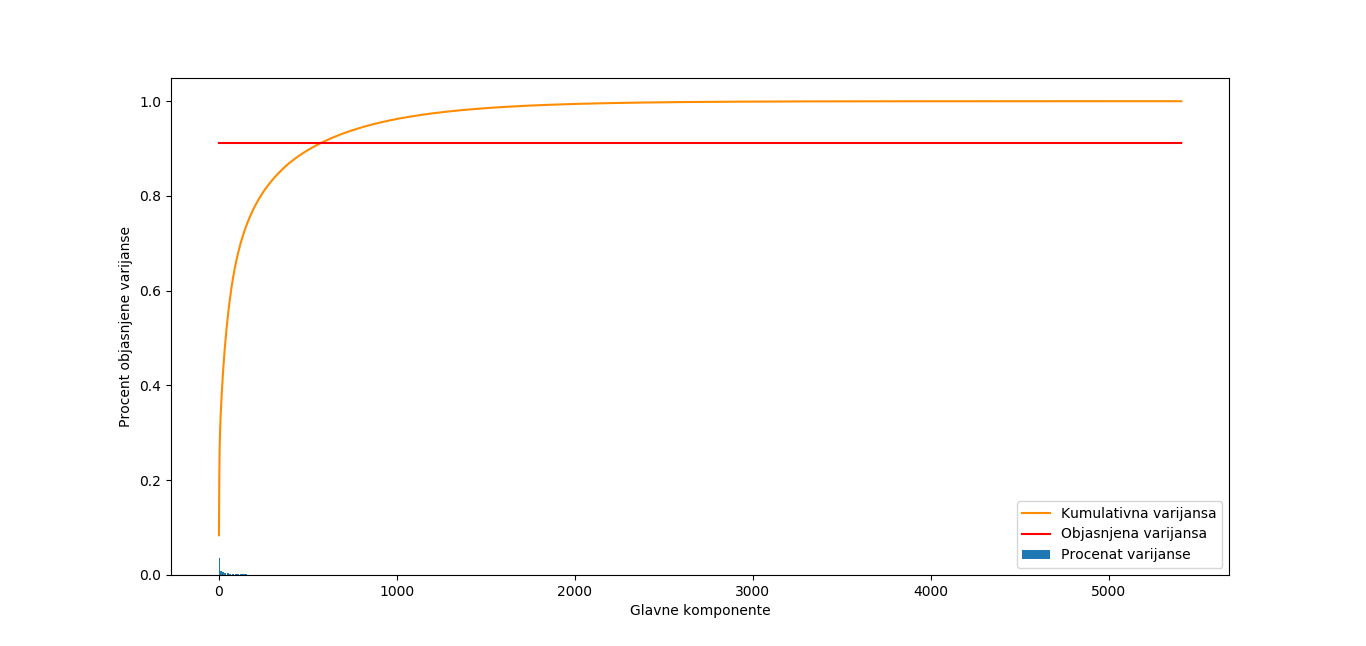
\includegraphics[width=0.7\textwidth]{img/pca.png}
    \caption{Matrica korelacije atributa}
    \label{fig:mesh1}
\end{figure}

\section {Modeliranje}

Obrada i analiza podataka se sastoji od sledećeg:

\begin{itemize}

	\item Izvesti obuku stabla odlučivanja nad skupom za obučavanje koji sadrži sve atribute dobijene PCA transformacijom i testirati dobijeni model na skupu za obučavanje i testiranje. Za implementaciju algoritma korišćen je model DecisionTreeClassifier iz biblioteke SciKit-Learn u jeziku Python.
	\item Primenom neuronske mreže izvršiti klasifikaciju nad transformisanim skupom podataka i predstaviti izveštaj klasifikacije. Za implementaciju neuronske mreže koristiti MLPClassifier klasu iz biblioteke SciKit-Learn. Takođe predstaviti strukturu rezultujuće mreže.
	\item Pomoću metoda potpornih vektora SVC iz biblioteke SciKit-Learn u jeziku Python kreirati model koji vrši klasifikaciju nad transformisanim skupom podataka i zatim uraditi izveštaj klasifikacije na skupu za treniranje i testiranje i utvrditi da li je došlo do preprilagoćavanja.

\end{itemize}

Prilikom izvođenja svakog od ovih eksperimenata primenjena je unakrsna validacija za izbor konfiguracije modela jer je uzeto u obzir više parametara i vrednosti parametara za treniranje modela. Za primenu unakrsne validacije korišćena je klasa GridSearchCV iz biblioteke SciKit-Learn, pri čemu broj podskupova podele skupa za obučavanje je bio postavljen na 5 u svakom od eksperimenata.

\subsection {Stablo odlučivanja}
Stablo odlučivanja predstavlja jednu od osnovnih tehnika za klasifikaciju podataka. Model klasifikacije dobijan ovom metodom je obično veoma jednostavan i lak za interpretaciju, jer opisuje proces klasifikacije na prirodan način. Svaki unutrašnji čvor u stablu predstavlja jednu podelu po određenom atributu, pri čemu svaki list predstavlja klasu koju taj list određuje. Dubina stabla opisuje koliko je model fleksibilan, odnosno koliko je podložan preprilagođavanju.

Za izgradnju stabla odlučivanja korišćen je ceo skup od 574 atributa jer veliki broj atributa u ovom slučaju ne može pokvariti interpretabilnost zbog samog nedostatka interpretabilnosti u prirodi atribut. Pored toga, urađena je i  PCA transformacije koja je oduzela i to malo interpretabilnosti što je na početku bilo prisutno. Isprobavani su različite kombinacije parametri konfiguracije stabla, tj. isprobavane su različite vrednosti parametara {\bf min-samples-split}, {\bf max-depth}, {\bf criterion}, {\bf max-leaf-nodes}, pri čemu najbolje se pokazala vrednost 2 za njamanju podelu uzorka, 5 za najveću dubinu stabla, dok je za maksimalan broj listova u stablu uzeta vrednost koja označava bez ograničenja a za ocenu mere nečistoće Ginijev indeks. Grafički prikaz stabla dobijenog jednom od isprobanih konfiguracija dat na slici 2.

\begin{figure}[h]
    \centering
    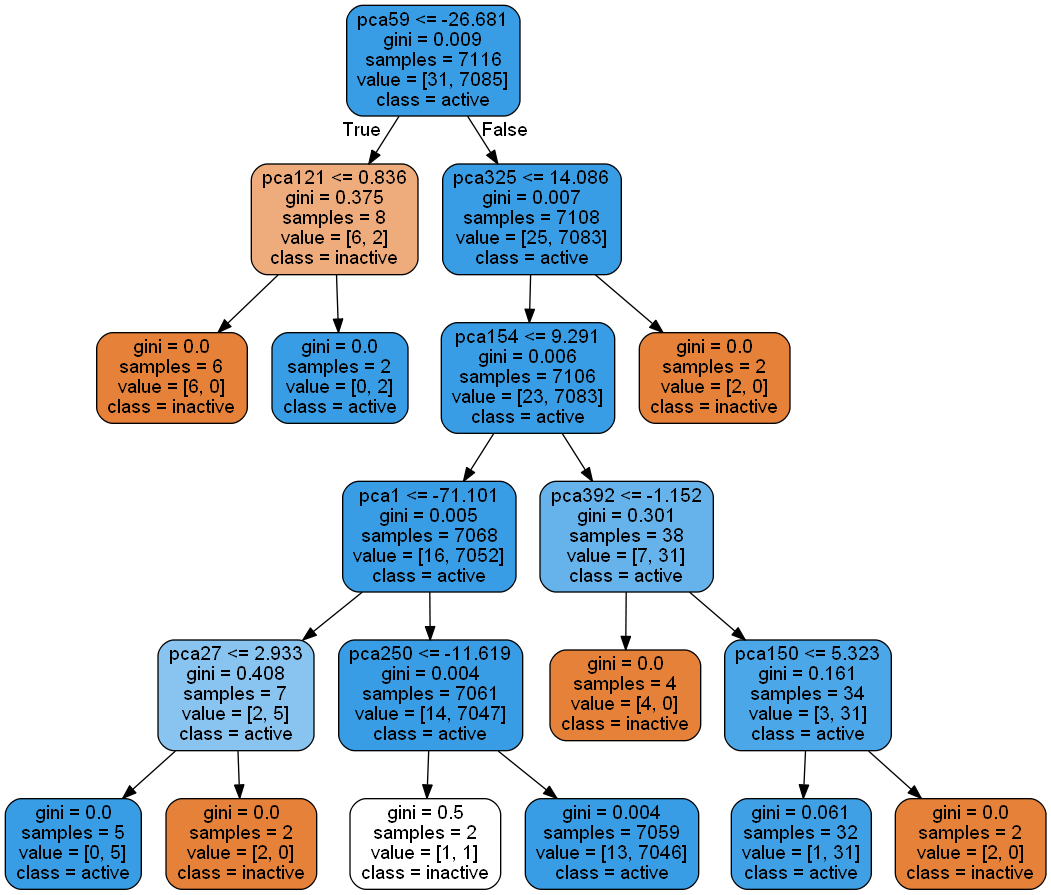
\includegraphics[width=0.7\textwidth]{img/tree.png}
    \caption{Grafički prikaz rezultujućeg stabla}
    \label{fig:mesh1}
\end{figure}

Na slici mogu se videti svaku od podela po atributima koje se vrše prilikom klasifikovanja novih instanci, svaki čvor sadrži informacije o atributu podele, oceni nečistoće čvorova, broju instanci trening skupa koje pripadaju posmatranom podstablu itd. Za pravljenje modela korišćen je ceo raspoloživ skup instanci jer pravljenje stabla odlučivanja nije toliko zahtevno po pitanju resursa, podela skupa instanci na trening skup i test skup je vršena u odnosu 2:1 respektivno za svaku od isprobanih konfiguracija modela. Najveća postignuta preciznost ovom metodom je 0.99, a ostali rezultati kao i ceo izvestaj klasifikacije optimalne konfiguracije stabla odlučivanja prikazani su u nastavku teksta tabelama 1, 2 i 3.  


\begin{table}
\caption{Matrica konfuzije Stabla Odlučivanja}
\centering
\begin{tabular}{|c|c|c|}
        	\hline
	& active & inactive \\
        	\hline
	active & 18 & 13 \\
	\hline
        	inactive & 4 & 7081 \\
	\hline
\end{tabular}
\end{table}

\begin{table}
\caption{Izveštaj klasifikacije Stabla Odlučivanja na skupu za obučavanje}
\centering
\begin{tabular}{|c|c|c|c|c|}
        	\hline
	& Precision & Recall & F1-Score & Support \\
        	\hline
	active & 0.94 & 0.55 & 0.69 & 31 \\
        	\hline
	inactive & 1.0 & 1.0 & 1.0 & 7085 \\
        	\hline
	Avg/Total & 1.0 & 1.0 & 1.0 & 7116 \\
	\hline
\end{tabular}
\end{table}

\begin{table}
\caption{Izveštaj klasifikacije Stabla Odlučivanja na skupu za testiranje}
\centering
\begin{tabular}{|c|c|c|c|c|}
        	\hline
	& Precision & Recall & F1-Score & Support \\
        	\hline
	active & 0.25 & 0.14 & 0.18 & 14 \\
        	\hline
	inactive & 1.0 & 1.0 & 1.0 & 3036 \\
        	\hline
	Avg/Total & 0.99 & 0.99 & 0.99 & 3050 \\
	\hline
\end{tabular}
\end{table}


\newpage
\subsection{Neuronska mreža}
Neuronska mreža predstavlja jednu od najprimenjenijih metoda mašinskog učenja. Najbolje rezultate pokazuje u domenima gde su ostale metode nemoćne a to je u slučajevima velikih skupova podataka i kada su podaci predstavljeni u sirovom obliku kao što je slučaj u ovom istraživanju.

Za definisanje strukture neuronske mreže koja je korišćena u ovom zadatku, izabrane su različite kombinacije vrednosti parametara kao što su  {\bf solver},  {\bf learning-rate},  {\bf learning-rate-init},  {\bf activation},  {\bf hidden-layer-sizes} i  {\bf max-iter}, pri čemu su vrednosti za parametre načina optimizacije i maksimalan broj iteracija bile fiksne, stohastički gradijentni spust i 500 iteracija respektivno. Nakon obučavanja svih modela, najbolje se pokazao model sa konfiguracijom: 


\begin{itemize}

	\item 'activation': 'tanh'
	\item 'hidden\_layer\_sizes': (10, 10)
	\item 'learning\_rate': 'adaptive'
	\item 'learning\_rate\_init': 0.01
	\item 'max\_iter': 500
	\item 'solver': 'sgd'

\end{itemize}

Za kreiranje ovog modela korišćen je ceo raspoloživ skup instanci, a podela skupa instanci na trening skup i test skup je vršena u odnosu 2:1 respektivno za svaku od isprobanih konfiguracija modela. Optimizacija je iskonvergirala nakon 69 iteracija a ukupan broj slojeva mreže je 4.  Najveća postignuta preciznost ovom metodom je 0.99, a ostali rezultati kao i ceo izvestaj klasifikacije optimalne konfiguracije neuronske mreže prikazani su u nastavku teksta tabelama 4 i 5.  


\begin{table}[h]
\caption{Matrica konfuzije najbolje neuronske mreže}
\centering
\begin{tabular}{|c|c|c|}
        	\hline
	& active & inactive \\
        	\hline
	active & 5 & 9 \\
	\hline
        	inactive & 4 & 3032  \\
	\hline
\end{tabular}
\end{table}


\begin{table}[h]
\caption{Izveštaj klasifikacije neuronske mreže na skupu za testiranje}
\centering
\begin{tabular}{|c|c|c|c|c|}
        	\hline
	& Precision & Recall & F1-Score & Support \\
        	\hline
	active & 0.56 & 0.36 & 0.43 & 14 \\
        	\hline
	inactive & 1.00 & 1.00 & 1.00 & 3036 \\
        	\hline
	Avg/Total & 1.00 & 1.00 & 1.00 & 3050 \\
	\hline
\end{tabular}
\end{table}

\subsection {Metod potpornih vektora}
Metod potpornih vektora predstavlja jendu od naprednijih metoda klasifikacije. Ideja je da se dati podaci klasifikuju tako što se razdvoje pomoću jedne ravni koja se zove razdvajajuća hiperravan. Postupak metode se sastoji od pretrage i optimizacije položaja razdvajajuće hiperravni kako bi se minimizovala ukupna greška pogrešno klasifikovanih podataka.

Za pretragu optimalne razdvajajuće hiperravni isprobavane su različite vrednosti parametara {\bf C},  {\bf kernel},  {\bf gamma},  {\bf coef0},  {\bf degree}. Za parametar regularizacije C uzeta je vrednost $2^x$, pri čemu su za $x$ uzete vrednosti iz skupa \{-6, -4, -2, 0, 2, 4, 6\}, dok su vrste korišćenih kernela Linearni, Gausov i Polinomijalni kernel. Koeficijent gama je uzimao vrednost iz skupa  \{0.1, 0.4, 0.7, 1.0\} a koeficijent coef0 iz skupa \{0, 0.5, 1.0\}. U nastavku su navedeni parametri optimalnog modela 

\begin{itemize}

	\item 'C': 16
	\item 'gamma': 0.1
	\item 'kernel': 'rbf''

\end{itemize}


Za obučavanje i testiranje modela metodom potpornih vektora korišćen je ceo skup podataka pri čemu je pre početka obučavanja vršena normalizacija podataka. Za svaku konfiguraciju raspoložive instance su podeljene ne trening i test skup u odnosu 2:1 respektivno. Klasifikacija je vršena na osnovu svih atributa izdvojenih u preprocesiranju i najveća postignuta preciznost je 0.99. Rezultati izvršavanja optimalne konfiguracije Metode Potpornih Vektora predstavljeno je tabelama 3 i 4, pri čemu je izostavljen prikaz rezultujućih vektora jer im je broj suviše veliki da bi bili pregledno prikazani u matrici. Matrica koja sadrži potprne vektore je dimenzije  [ 27 116]

\begin{table}[h]
\caption{Matrica konfuzije Metode Potpornih Vektora}
\centering
\begin{tabular}{|c|c|c|}
        	\hline
	& active & inactive \\
        	\hline
	active & 7 & 7 \\
	\hline
        	inactive & 7 & 3029  \\
	\hline
\end{tabular}
\end{table}

%Preciznost:  POMOĆU STRATEGIJE JEDAN-PROTIV-JEDNOG

\begin{table}[h]
\caption{Izveštaj klasifikacije Metode Potpornih Vektora na skupu za obučavanje}
\centering
\begin{tabular}{|c|c|c|c|c|}
        	\hline
	& Precision & Recall & F1-Score & Support \\
        	\hline
	active & 1.00 & 0.78 & 0.88 & 27 \\
        	\hline
	inactive & 1.00 & 1.00 & 1.00 & 7089 \\
        	\hline
	Avg/Total & 1.00 & 1.00 & 1.00 & 7116 \\
	\hline
\end{tabular}
\end{table}


\begin{table}
\caption{Izveštaj klasifikacije Metode Potpornih Vektora na skupu za testiranje}
\centering
\begin{tabular}{|c|c|c|c|c|}
        	\hline
	& Precision & Recall & F1-Score & Support \\
        	\hline
	active & 0.56 & 0.28 & 0.37 & 18 \\
        	\hline
	inactive & 1.00 & 1.00 & 1.00 & 3032 \\
        	\hline
	Avg/Total & 0.99 & 0.99 & 0.99 & 3050 \\
	\hline
\end{tabular}
\end{table}


\newpage
\section {Evaluacija modela i analiza rezultata}
Prilikom poređenja rezultata metoda pri različitim parametrima modela, kao i poređenja rezultata različitih metoda, utvrđeno je da su sve instance metoda pokazale isti ili veoma sličan uspeh. To dalje nagoveštava da su metode najverovatnije postigle najviše što je moglo da se isporuči na osnovu datih podataka. Primećeno je i preprilagođavanje kod sve tri modela što je i bilo očekivano jer je skup podataka pristrasan klasi "inactive", tj. skup podataka sadrži jako mali broj primera klase "active". Takođe se može zaključiti da je sama uslovljenost ovog problema veoma loša pa je zbog toga i pouzdanost ovih rezultata veoma niska. 

\section {Zaključak}
Predmet proučavanja u ovom radu bila je baza podataka koja sadrži informacije biofizičkim modelima p53 gena. Cilj je bio da se kreira model koji bi pomogao u identifikaciji neaktivnih p53 gena. Za ostvarivanje tog cilja isprobavane su razne tehnike, alati i algoritmi istrazivanja podataka i mašinskog učenja, neke od njih su klasifikacija primenom Stabla Odlučivanja i Metode Potpornih Vektora i Neuronske Mreže na skript jeziku Python pomoću biblioteke SciKit-Learn. Takođe su razmatrane i druge tehnike poput klasifikacije kao što je algoritam k najbližih suseda i Bajesov klasifikator, međutim, ovi algoritmi su odbačeni jer priroda podataka nije pogodna za njihovu primenu. Naime, visoka dimenzionalnost i neprekidna priroda atributa su dve velike prepreke za ove dve metode.\end{document}



